\chapter{Regió lliure de zeros (de $\zeta$, dins de la franja crítica).}
\teorema{Regió lliure de zeros}{\label{6.01_teorema regió lliure de zeros}Existeix una $c\in\RR_{>0}$ tal que els zeros no trivials de $\zeta$ pertanyen a la següent regió.
\[
    \frac{c}{\log(2+|t|)}\leq \s\leq 1-\frac{c}{\log(2+|t|)}
\]}

\begin{wrapfigure}{r}{0.25\textwidth}
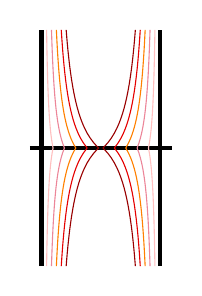
\begin{tikzpicture}[domain=0:3, scale=0.5]
    \draw[ultra thick] (-0.3,0)--(3.3,0);
    \draw[ultra thick] (0,-3)--(0,3);
    \draw[ultra thick] (3,-3)--(3,3);
    \draw[red!60!black] plot (   {1/(ln(2+\x))},    \x);
    \draw[red!60!black] plot ({3-(1/(ln(2+\x)))},   \x);
    \draw[red!60!black] plot (   {1/(ln(2+\x))},    {-\x});
    \draw[red!60!black] plot ({3-(1/(ln(2+\x)))},   {-\x});
    %
    \draw[red!90!black] plot (   {0.8/(ln(2+\x))},    \x);
    \draw[red!90!black] plot ({3-(0.8/(ln(2+\x)))},   \x);
    \draw[red!90!black] plot (   {0.8/(ln(2+\x))},    {-\x});
    \draw[red!90!black] plot ({3-(0.8/(ln(2+\x)))},   {-\x});
    %
    \draw[orange] plot (   {0.6/(ln(2+\x))},    \x);
    \draw[orange] plot ({3-(0.6/(ln(2+\x)))},   \x);
    \draw[orange] plot (   {0.6/(ln(2+\x))},    {-\x});
    \draw[orange] plot ({3-(0.6/(ln(2+\x)))},   {-\x});
    %
    \draw[pink!70!purple] plot (   {0.4/(ln(2+\x))},    \x);
    \draw[pink!70!purple] plot ({3-(0.4/(ln(2+\x)))},   \x);
    \draw[pink!70!purple] plot (   {0.4/(ln(2+\x))},    {-\x});
    \draw[pink!70!purple] plot ({3-(0.4/(ln(2+\x)))},   {-\x});
    %
    \draw[pink] plot (   {0.2/(ln(2+\x))},    \x);
    \draw[pink] plot ({3-(0.2/(ln(2+\x)))},   \x);
    \draw[pink] plot (   {0.2/(ln(2+\x))},    {-\x});
    \draw[pink] plot ({3-(0.2/(ln(2+\x)))},   {-\x});
\end{tikzpicture}
% \begin{tikzpicture}[domain=0:4]
%   \draw[very thin,color=gray] (-0.1,-1.1) grid (3.9,3.9);

%   \draw[->] (-0.2,0) -- (4.2,0) node[right] {$x$};
%   \draw[->] (0,-1.2) -- (0,4.2) node[above] {$f(x)$};

%   \draw[color=red]    plot (\x,\x)             node[right] {$f(x) =x$};
%   % \x r means to convert '\x' from degrees to _r_adians:
%   \draw[color=blue]   plot (\x,{sin(\x r)})    node[right] {$f(x) = \sin x$};
%   \draw[color=orange] plot (\x,{0.05*exp(\x)}) node[right] {$f(x) = \frac{1}{20} \mathrm e^x$};
% \end{tikzpicture}
\end{wrapfigure}
Podem graficar la següent regió per diferents valors de $c$, i ens dona el següent:\\
Encara no farem la demostració d'aquest teorema; però de la mateixa manera que la funció $L(\chi,s)$ tingués un pol en $s=1$ era un punt clau de la demostració del teorema de Dirichlet per a successions; aquest teorema serà de vital importància per la demostració del teorema del nombre primer.
\vspace{7mm}
\lema{}{\label{6.02_lema}Per $\s>1$ es té:
\begin{enumerate}
    \ii $\Re\;\log(\zeta(s))=\sum_p\sum_{m\geq1}\frac{\cos(mt)\log p}{mp^{\s m}}$\\
    \ii $-\Re\; \frac{\zeta'(s)}{\zeta(s)}=\sum_{n\geq1}\frac{\Lambda(n)\,\cos(t\log n)}{n^\s}$.
\end{enumerate}
On en el segon apartat, la funció $\Lambda(n)=\left\{\begin{array}{cc}
    \log p&\text{ si }n=p^k\\
    0&\text{ altrament.}
\end{array}\right.$
}
\pf{
Per $s\in\RR_{>1}$ ja sabem del corol·lari $\ref{2.17_coro sèries de potències de p}$ del capítol \ref{capítol 1: sèries de Dirichlet}, que 
\[
    \log(\zeta(s))=-\sum_{p}\log(1-p^{-s})=\sum_p\sum_{m\geq 1}\frac{1}{mp^{\s m}}
\]
I per continuació analítica, la igualtat es certa per $s=\s+it\in \CC$. Per tant:
\[
    \log(\zeta(s))=\sum_p\sum_{m\geq1}\frac{1}{mp^{ms}}=\sum_p\sum_{m\geq1}\frac{p^{-im t}}{mp^{m\s}}
\]
I ara, si prenem la part real del que tenim:
\[
    \Re\,\log(\zeta(s))=\sum_p\sum_{m\geq1}\frac{\cos(mt)\log p}{mp^{m\s}}
\]
On la igualtat ve de que si $\theta\in\RR$, aleshores $p^{i\theta}=\log p(\cos(\theta)+i\sin(\theta))$.
Que és el que volíem veure pel primer apartat.\\
Pel segon, notem que $\frac{\zeta'(s)}{\zeta(s)}$ és la derivada logarítmica de $\zeta(s)$, per tant:
\[
    \frac{\zeta'(s)}{\zeta(s)}=
    \left(-\sum_p\sum_{m\geq1}\frac{1}{mp^{ms}}\right)'\overset{(*)}{=}
    \sum_p\sum_{m\geq1}\frac{\log(p)}{p^{ms}}=-\sum_{n\geq1}\frac{\Lambda(n)}{n^s}
\]
On $(*)$ ve de que tenim convergència absoluta. I ara si estudiem la part real:
\[
    \Re\left(\frac{\zeta'(s)}{\zeta(s)}\right)=
    -\sum_{n\geq1}\frac{\cos(t\log(n))\Lambda(n)}{n^s}
\]
Que és el que necessitem veure.
}
I ara, degut a que han aparegut funcions trigonomètriques, voldrem tenir algun control sobre aquestes; i d'aquí sorgirà el lema de Mertens:
\lema{Lema de Mertens}{\label{6.03_lema de Mertens} Per qualsevol $\theta\in\RR$, tenim la següent desigualtat.
\[
    3+4\cos(\theta)+\cos(2\theta)\geq0
\]
}
\pf{
Utilitzant la fórmula de l'angle doble del cosinus, tenim:
\[
    3+4\cos(\theta)+\cos(2\theta)=
    3+4\cos(\theta)+\cos^2(\theta)-\sin^2(\theta)=
    2(1+\cos(\theta))^2\geq0
\]
}
I ara d'aquesta identitat trigonomètrica se'n poden derivar dos sobre la funció $\zeta$:
\Prop{Mertens per a la funció $\zeta$.}{
    Per $\s>1$, tenim:
    \begin{enumerate}
        \ii $\zeta^3(\s)|\zeta^4(\s+it)||\zeta(\s+i2t)|\geq0$,\\
        \ii $3\left(-\frac{\zeta'(\s)}{\zeta(\s)}\right)+4\Re\left(\frac{\zeta'(\s+it)}{\zeta(\s+it)}\right)+3\left(-\frac{\zeta'(\s+i2t)}{\zeta(\s+i2t)}\right)\geq0$.
    \end{enumerate}
}